\documentclass[border=10pt]{standalone}

\usepackage{tikz}
\usepackage{tikzsymbols}
\usetikzlibrary{calc,patterns,shapes.geometric}

\def\centerarc[#1](#2)(#3:#4:#5){\draw[#1] ($(#2)+({#5*cos(#3)},{#5*sin(#3)})$) arc (#3:#4:#5);}

\begin{document}
	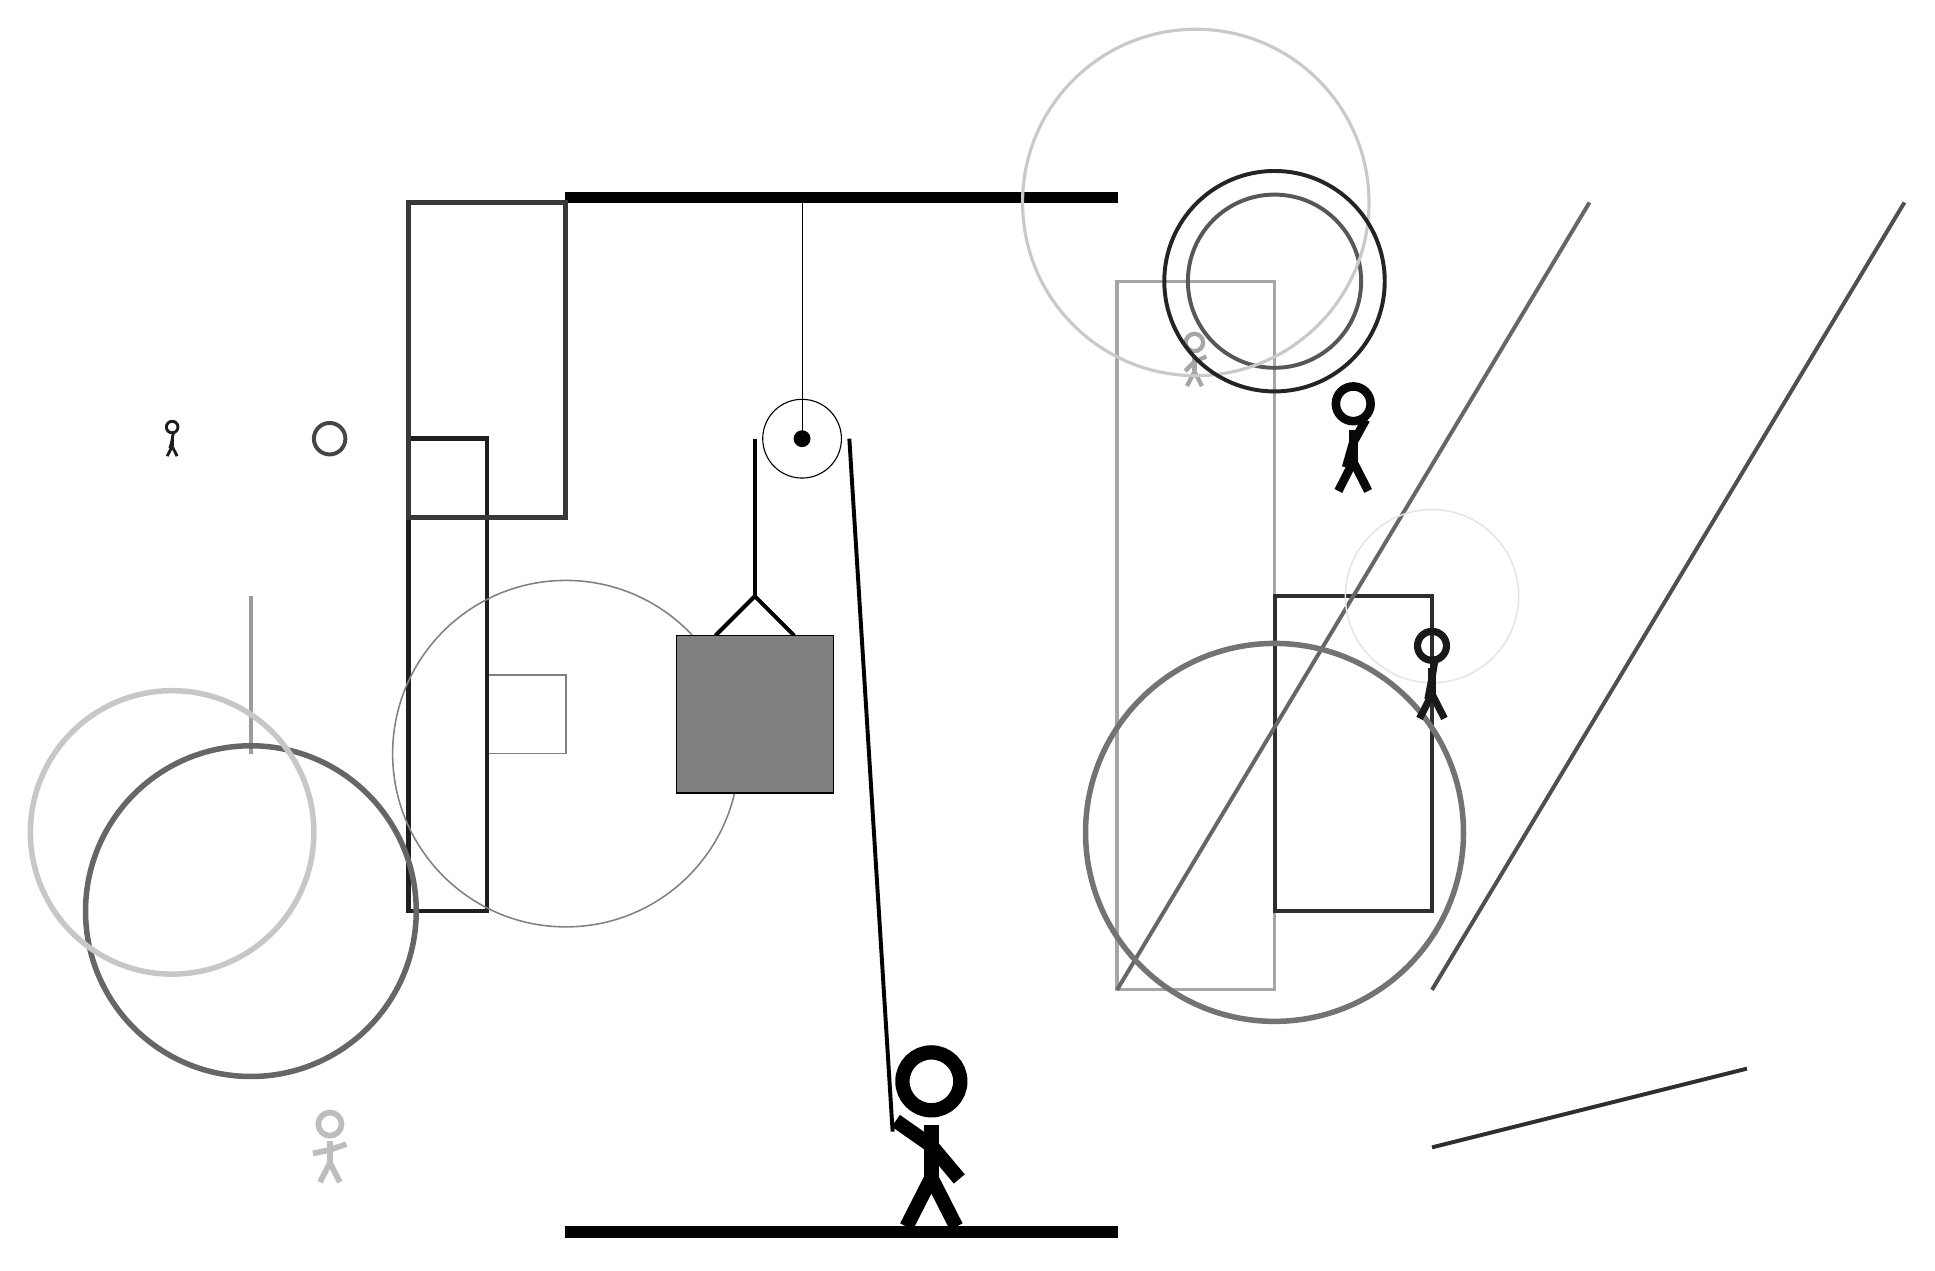
\begin{tikzpicture}
		%%%%% START %%%%%
		
		\draw[fill=black] (-2, 10) rectangle (5, 10.125);
		
		\draw (1, 7) circle (0.5);
		\draw[fill=black] (1, 7) circle (0.1);
		\draw (1, 10) -- (1, 7);
		
		\draw [line width=0.5mm, color=black!73](-5, 7) circle (0.2);
		
		\node[line width=0.7mm, color=black!26] at (-5, -2) {\Strichmaxerl[4][12][19]};
		\draw[line width=0.2mm, color=black!50] (-2, 3) rectangle (-3, 4);
		\node[line width=0.6mm, color=black!89] at (-7, 7) {\Strichmaxerl[2][75][81]};
		\draw[line width=0.4mm, color=black!35] (5, 9) rectangle (7, 0);
		
		\node[line width=0.3mm, color=black!35] at (6, 8) {\Strichmaxerl[3][45][24]};
		
		\node[line width=0.3mm, color=black!97] at (8, 7) {\Strichmaxerl[6][74][61]};
		
		\draw [line width=0.5mm, color=black!66](7, 9) circle (1.1);
		\draw[line width=0.5mm, color=black!82] (7, 1) rectangle (9, 5);
		
		\draw[line width=0.5mm, color=black!39](-6, 5) -- (-6, 3);
		\draw[line width=0.5mm, color=black!60](5, 0) -- (11, 10);
		
		\draw[line width=0.5mm, color=black!69](9, 0) -- (15, 10);
		\draw[line width=0.6mm, color=black!88] (-4, 7) rectangle (-3, 1);
		
		\draw [line width=0.4mm, color=black!21](6, 10) circle (2.2);
		\draw [line width=0.5mm, color=black!86](7, 9) circle (1.4);
		\draw[line width=0.5mm, color=black!82](9, -2) -- (13, -1);
		
		\draw [line width=0.7mm, color=black!60](-6, 1) circle (2.1);
		
		\draw [line width=0.2mm, color=black!10](9, 5) circle (1.1);
		\draw[line width=0.6mm, color=black!78] (-2, 10) rectangle (-4, 6);
		\draw [line width=0.7mm, color=black!55](7, 2) circle (2.4);
		\draw [line width=0.7mm, color=black!22](-7, 2) circle (1.8);
		
		\node[line width=0.3mm, color=black!90] at (9, 4) {\Strichmaxerl[5][79][81]};
		\draw [line width=0.2mm, color=black!49](-2, 3) circle (2.2);
		
		\draw[line width=0.5mm] (-0.1, 4.5) -- (0.4, 5.0) -- (0.9, 4.5);
		\draw[fill=black!50] (-0.6, 4.5) rectangle (1.4, 2.5);
		
		\draw[line width=0.5mm] (0.4, 7) -- (0.4, 5.0);
		\centerarc[line width=0.5mm](1, 7)(0:180:0.6);
		\draw[line width=0.5mm](1.6, 7) -- (2.15, -1.8);
		
		\node at (2.6, -1.9) {\Strichmaxerl[10][-35][-50]};
		
		\draw[fill=black] (-2, -3) rectangle (5, -3.15);
		
		%%%%% END %%%%%
	\end{tikzpicture}
\end{document}